\unchapter{Conclusioni}

%--------------------------------------------------------------------------------------------

\unsection{Suddivisione delle Schede}

%--------------------------------------------------------------------------------------------

Ogni blocco discusso finora viene collegato assieme secondo il seguente schema:

\begin{figure}[H]
    \centering
    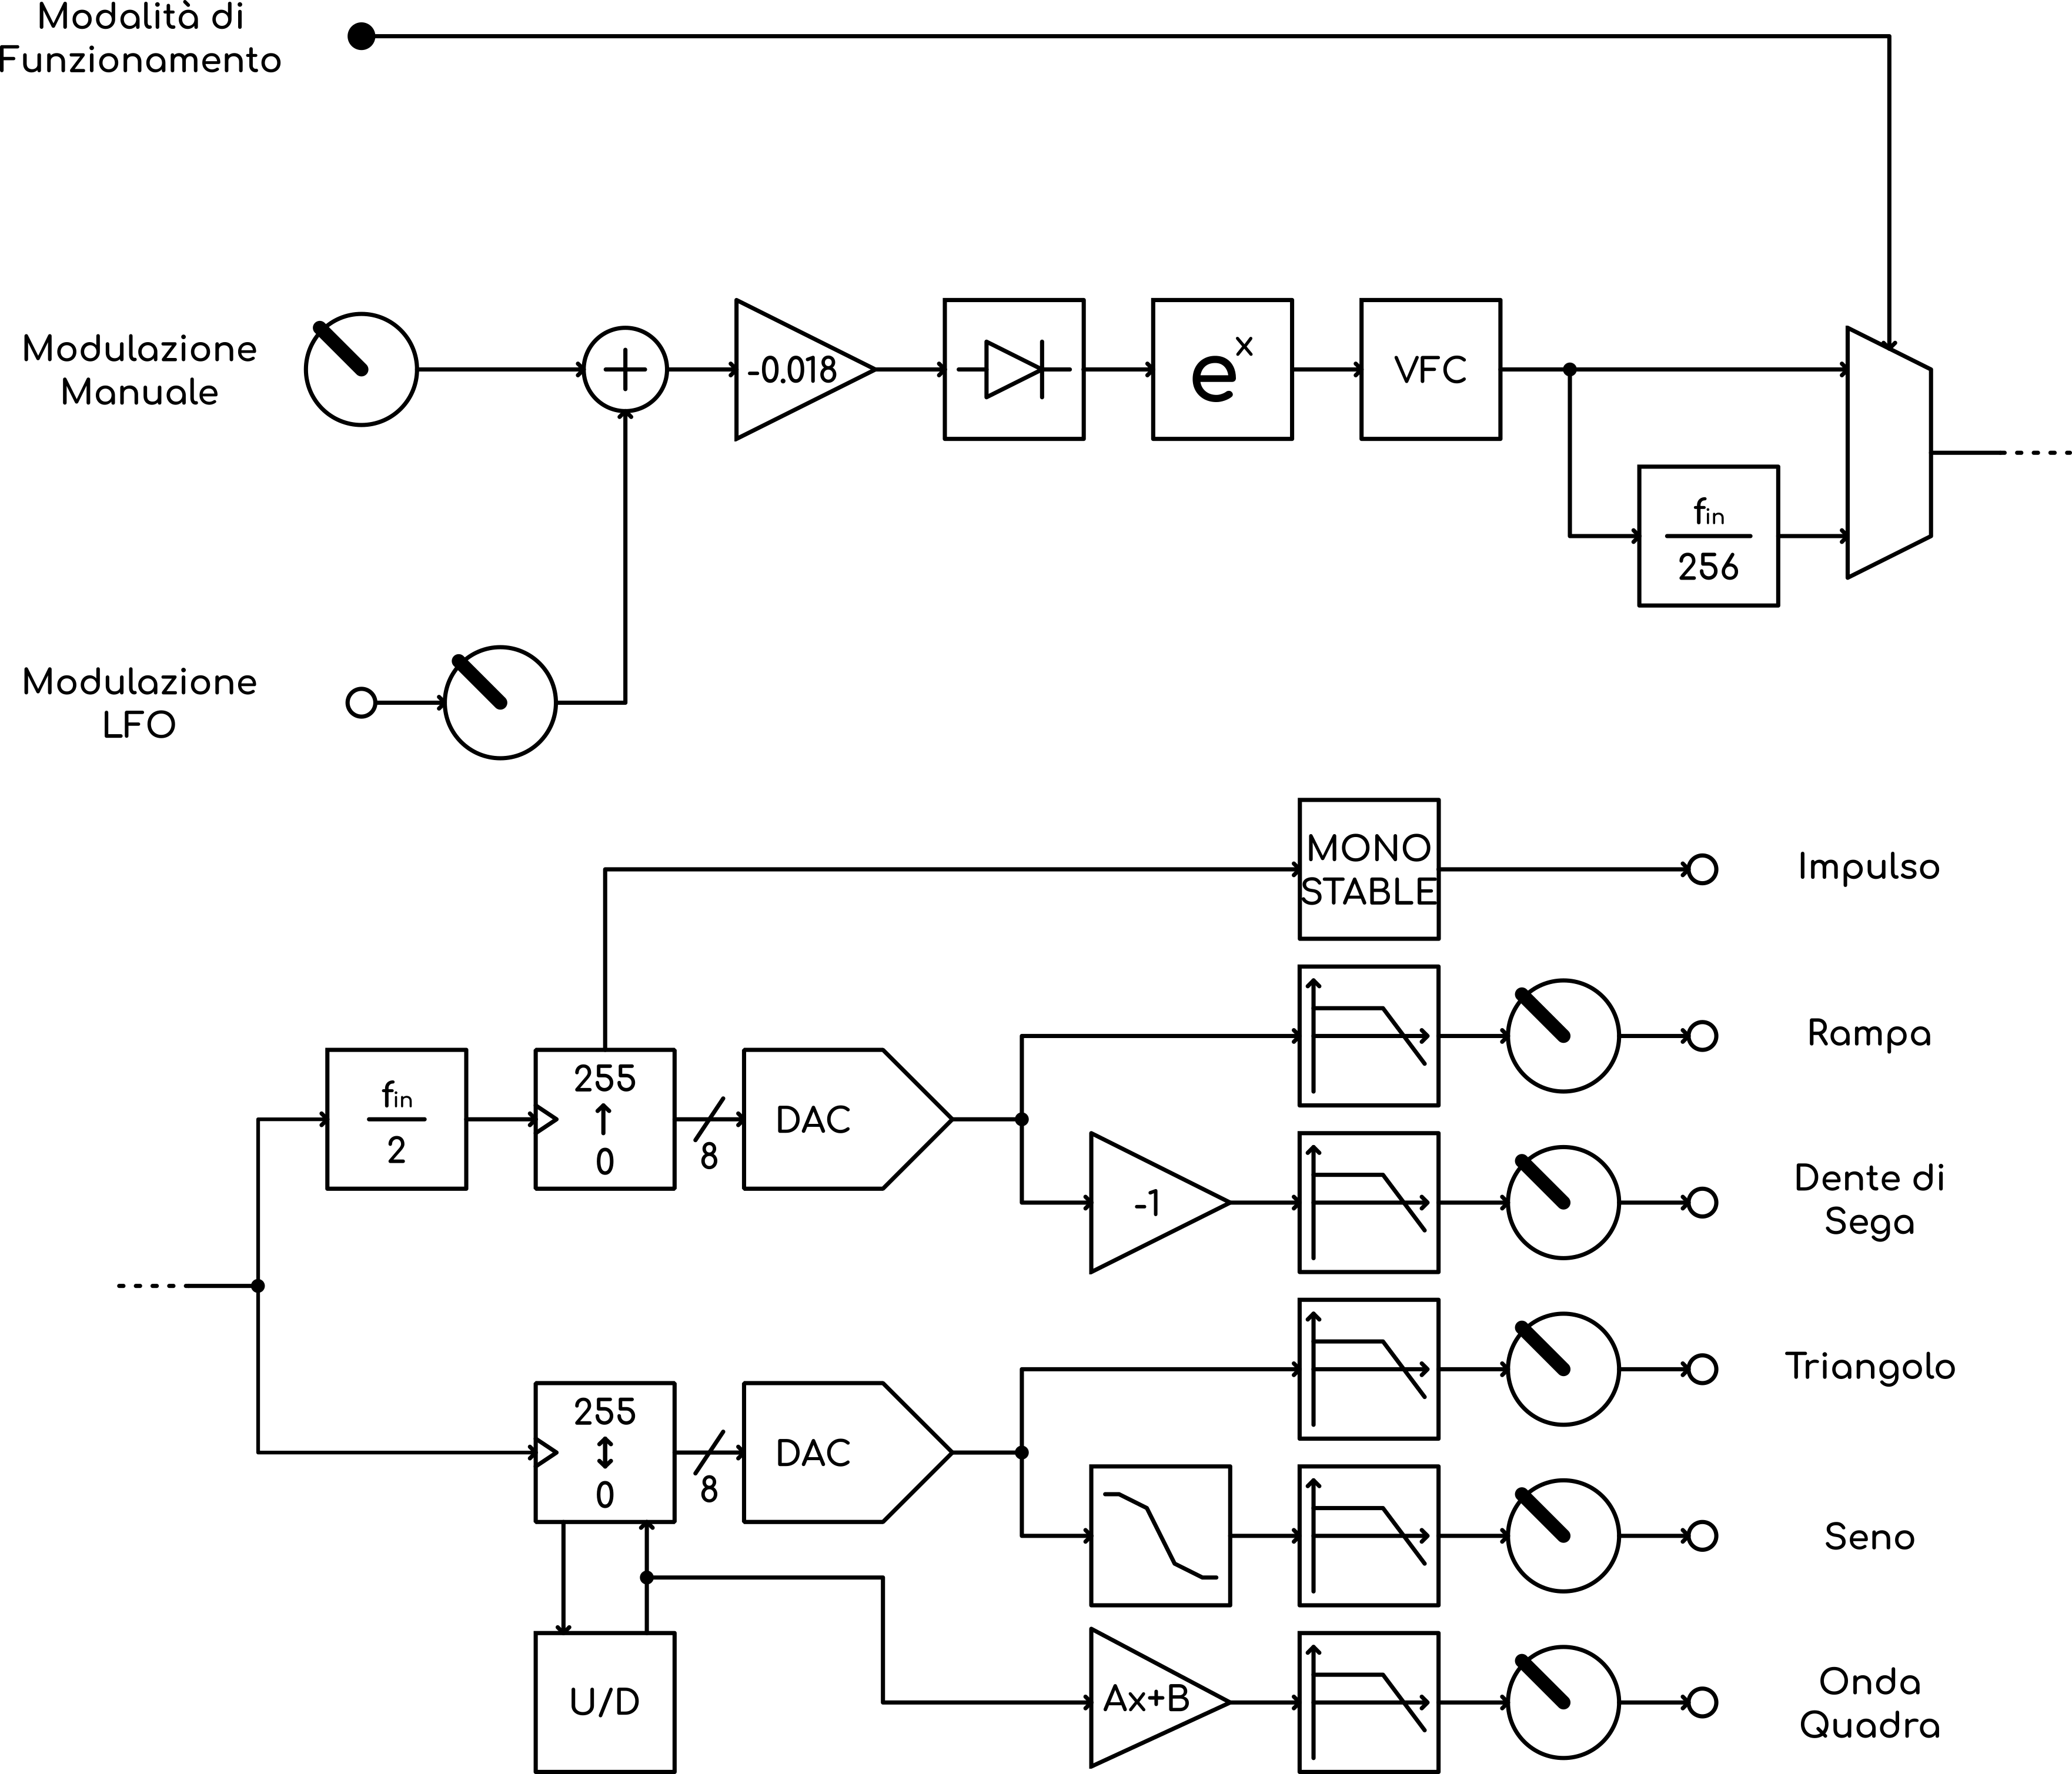
\includegraphics[scale = 0.5]{block_diagrams/full_block_diagram.png}
    \caption{Schema a blocchi completo}
    \label{full_block_diagram}
\end{figure}

Si suddivide poi l'intero circuito in un totale di 3 schede, in modo da ridurre al
minimo l'ingombro del modulo e non avere delle schede troppo dense di componenti.

\begin{figure}[H]
    \centering
    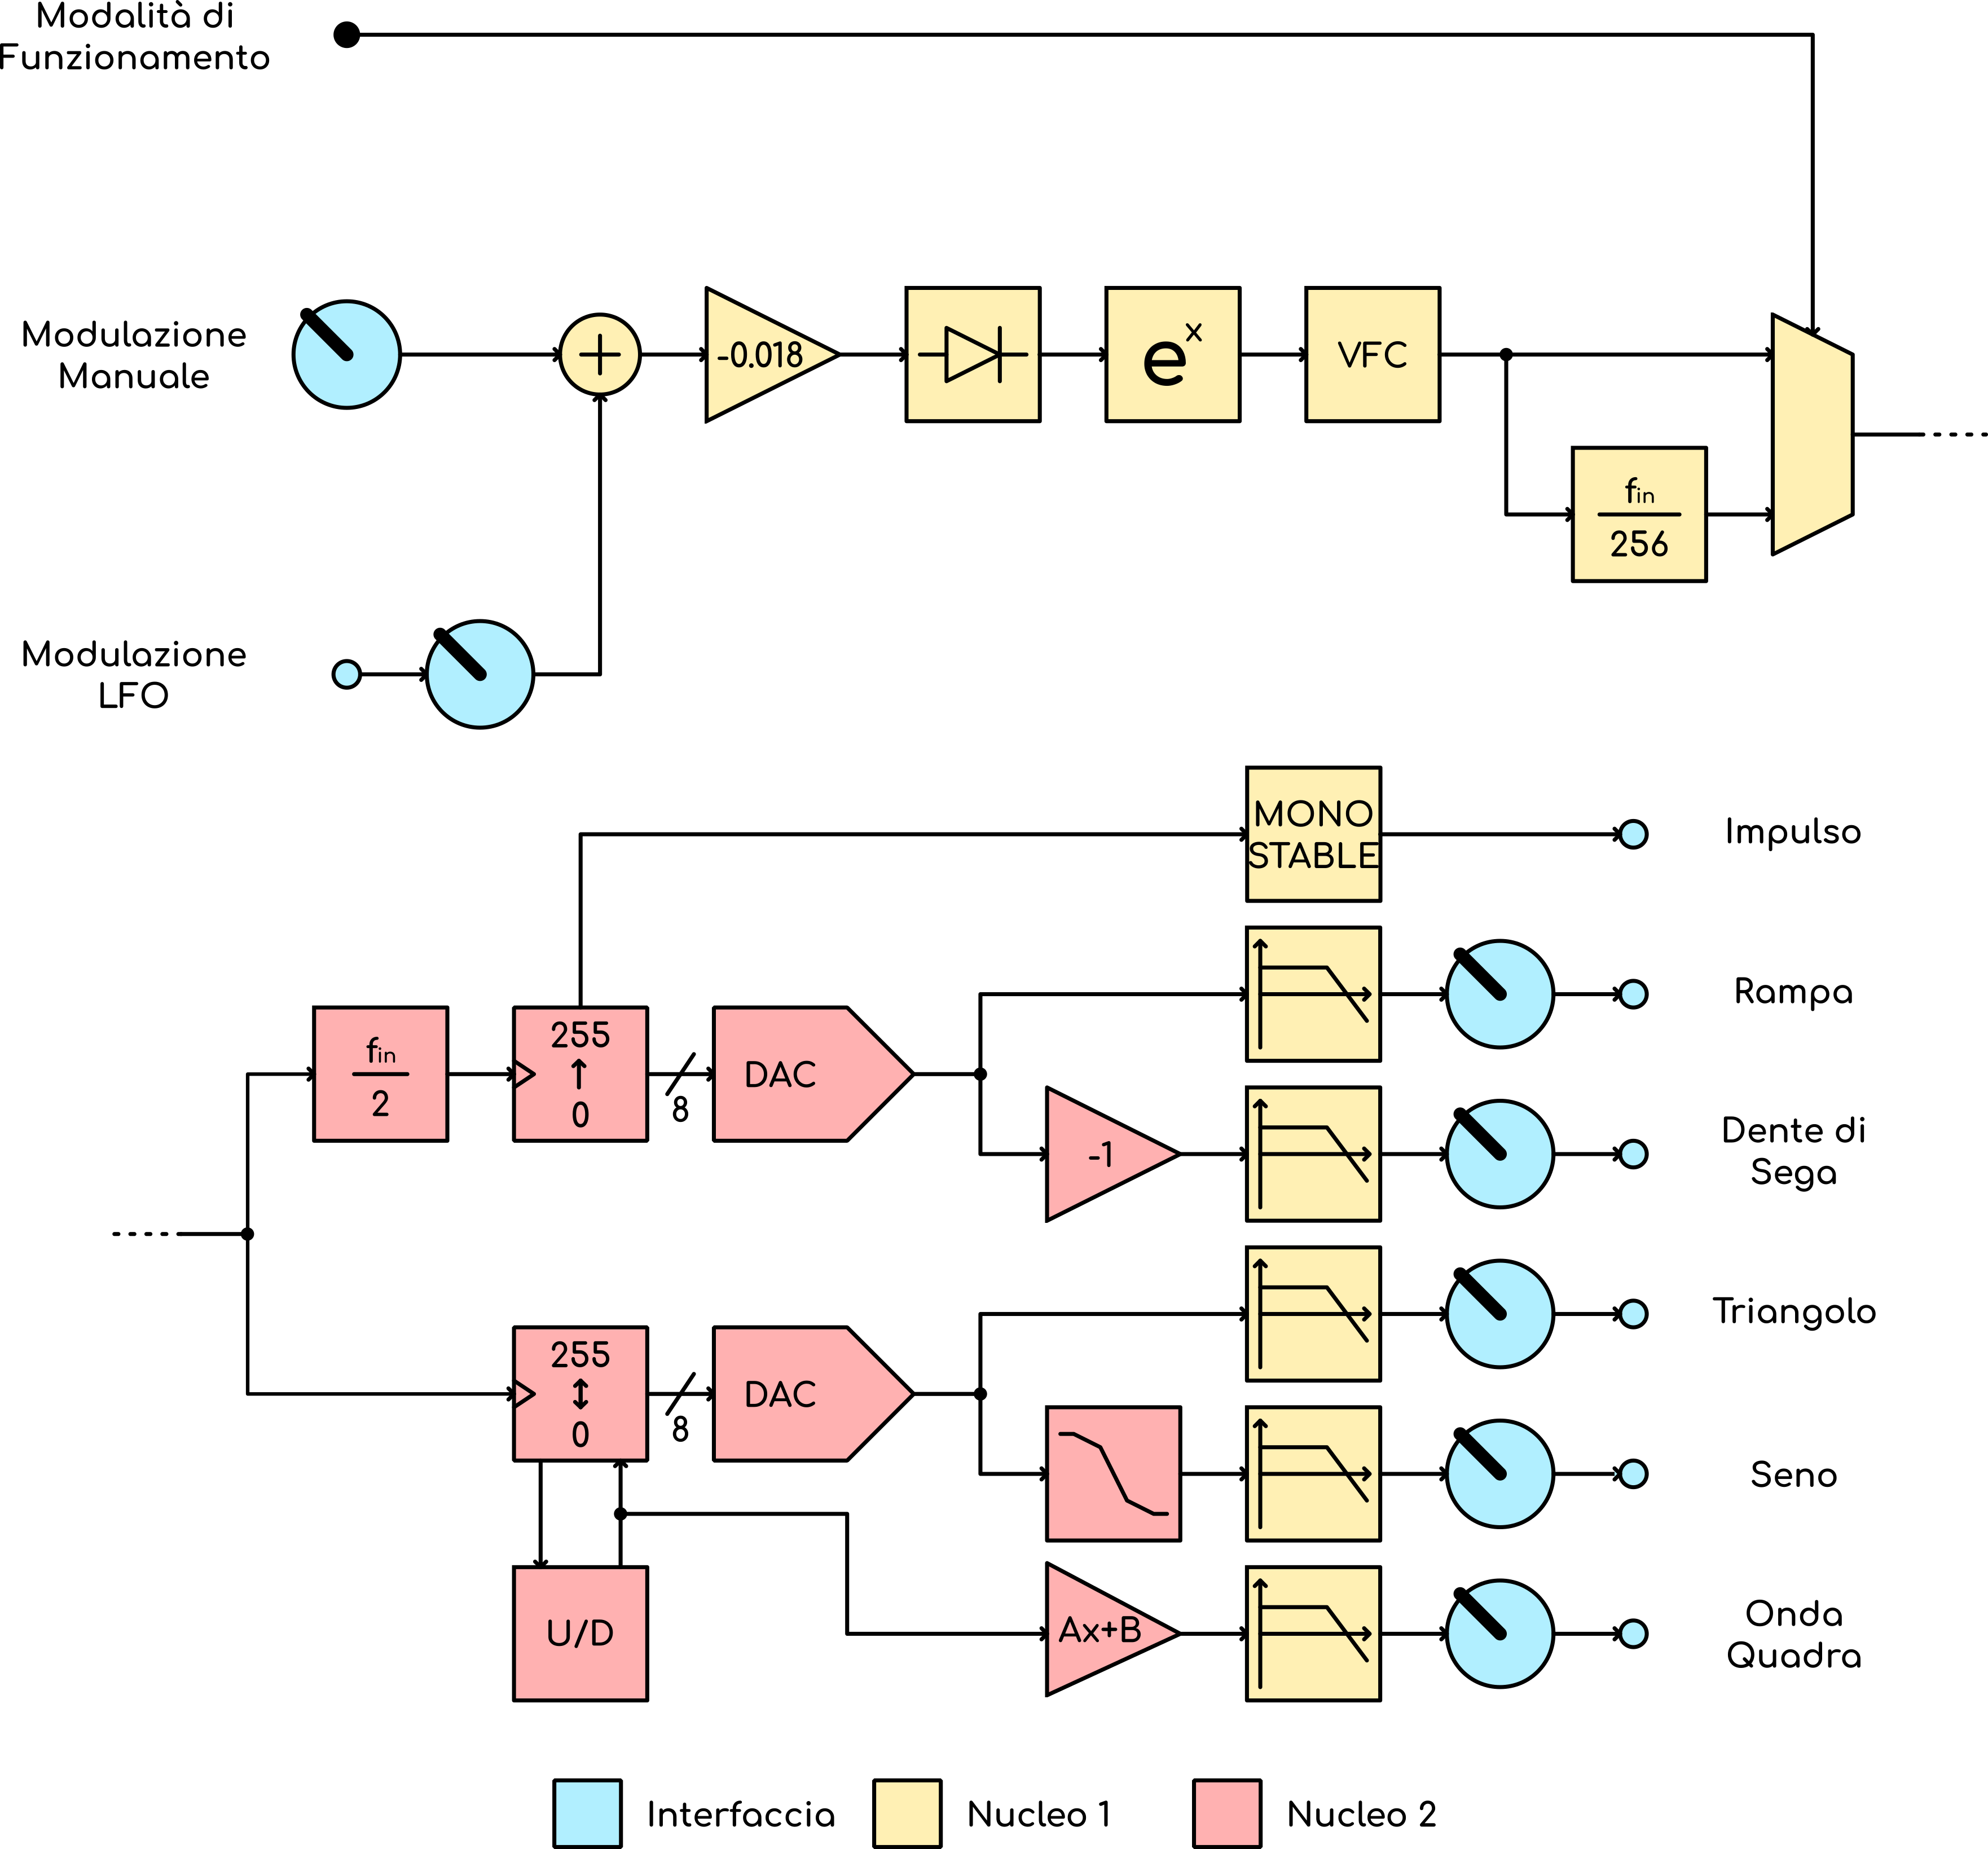
\includegraphics[scale = 0.5]{block_diagrams/full_block_diagram_colored.png}
    \caption{Suddivisione dei blocchi nelle varie schede}
    \label{full_block_diagram_colored}
\end{figure}

Le schede verranno impilate una sopra l'altra e collegate tra loro con degli appositi connettori.
L'interfaccia mostrata in figura \ref{panel_explained} sarà effettivamente il pannello
frontale del nostro modulo, subito sotto andrà la scheda di interfaccia, la quale ospiterà
tutti i componenti atti all'interazione con l'utente e gli altri moduli (manopole, connettori
jack, LED, interruttori, ecc...). Nelle altre due schede invece si collocherà tutto il resto
del circuito secondo quanto specificato in figura.

\begin{figure}[H]
    \centering
    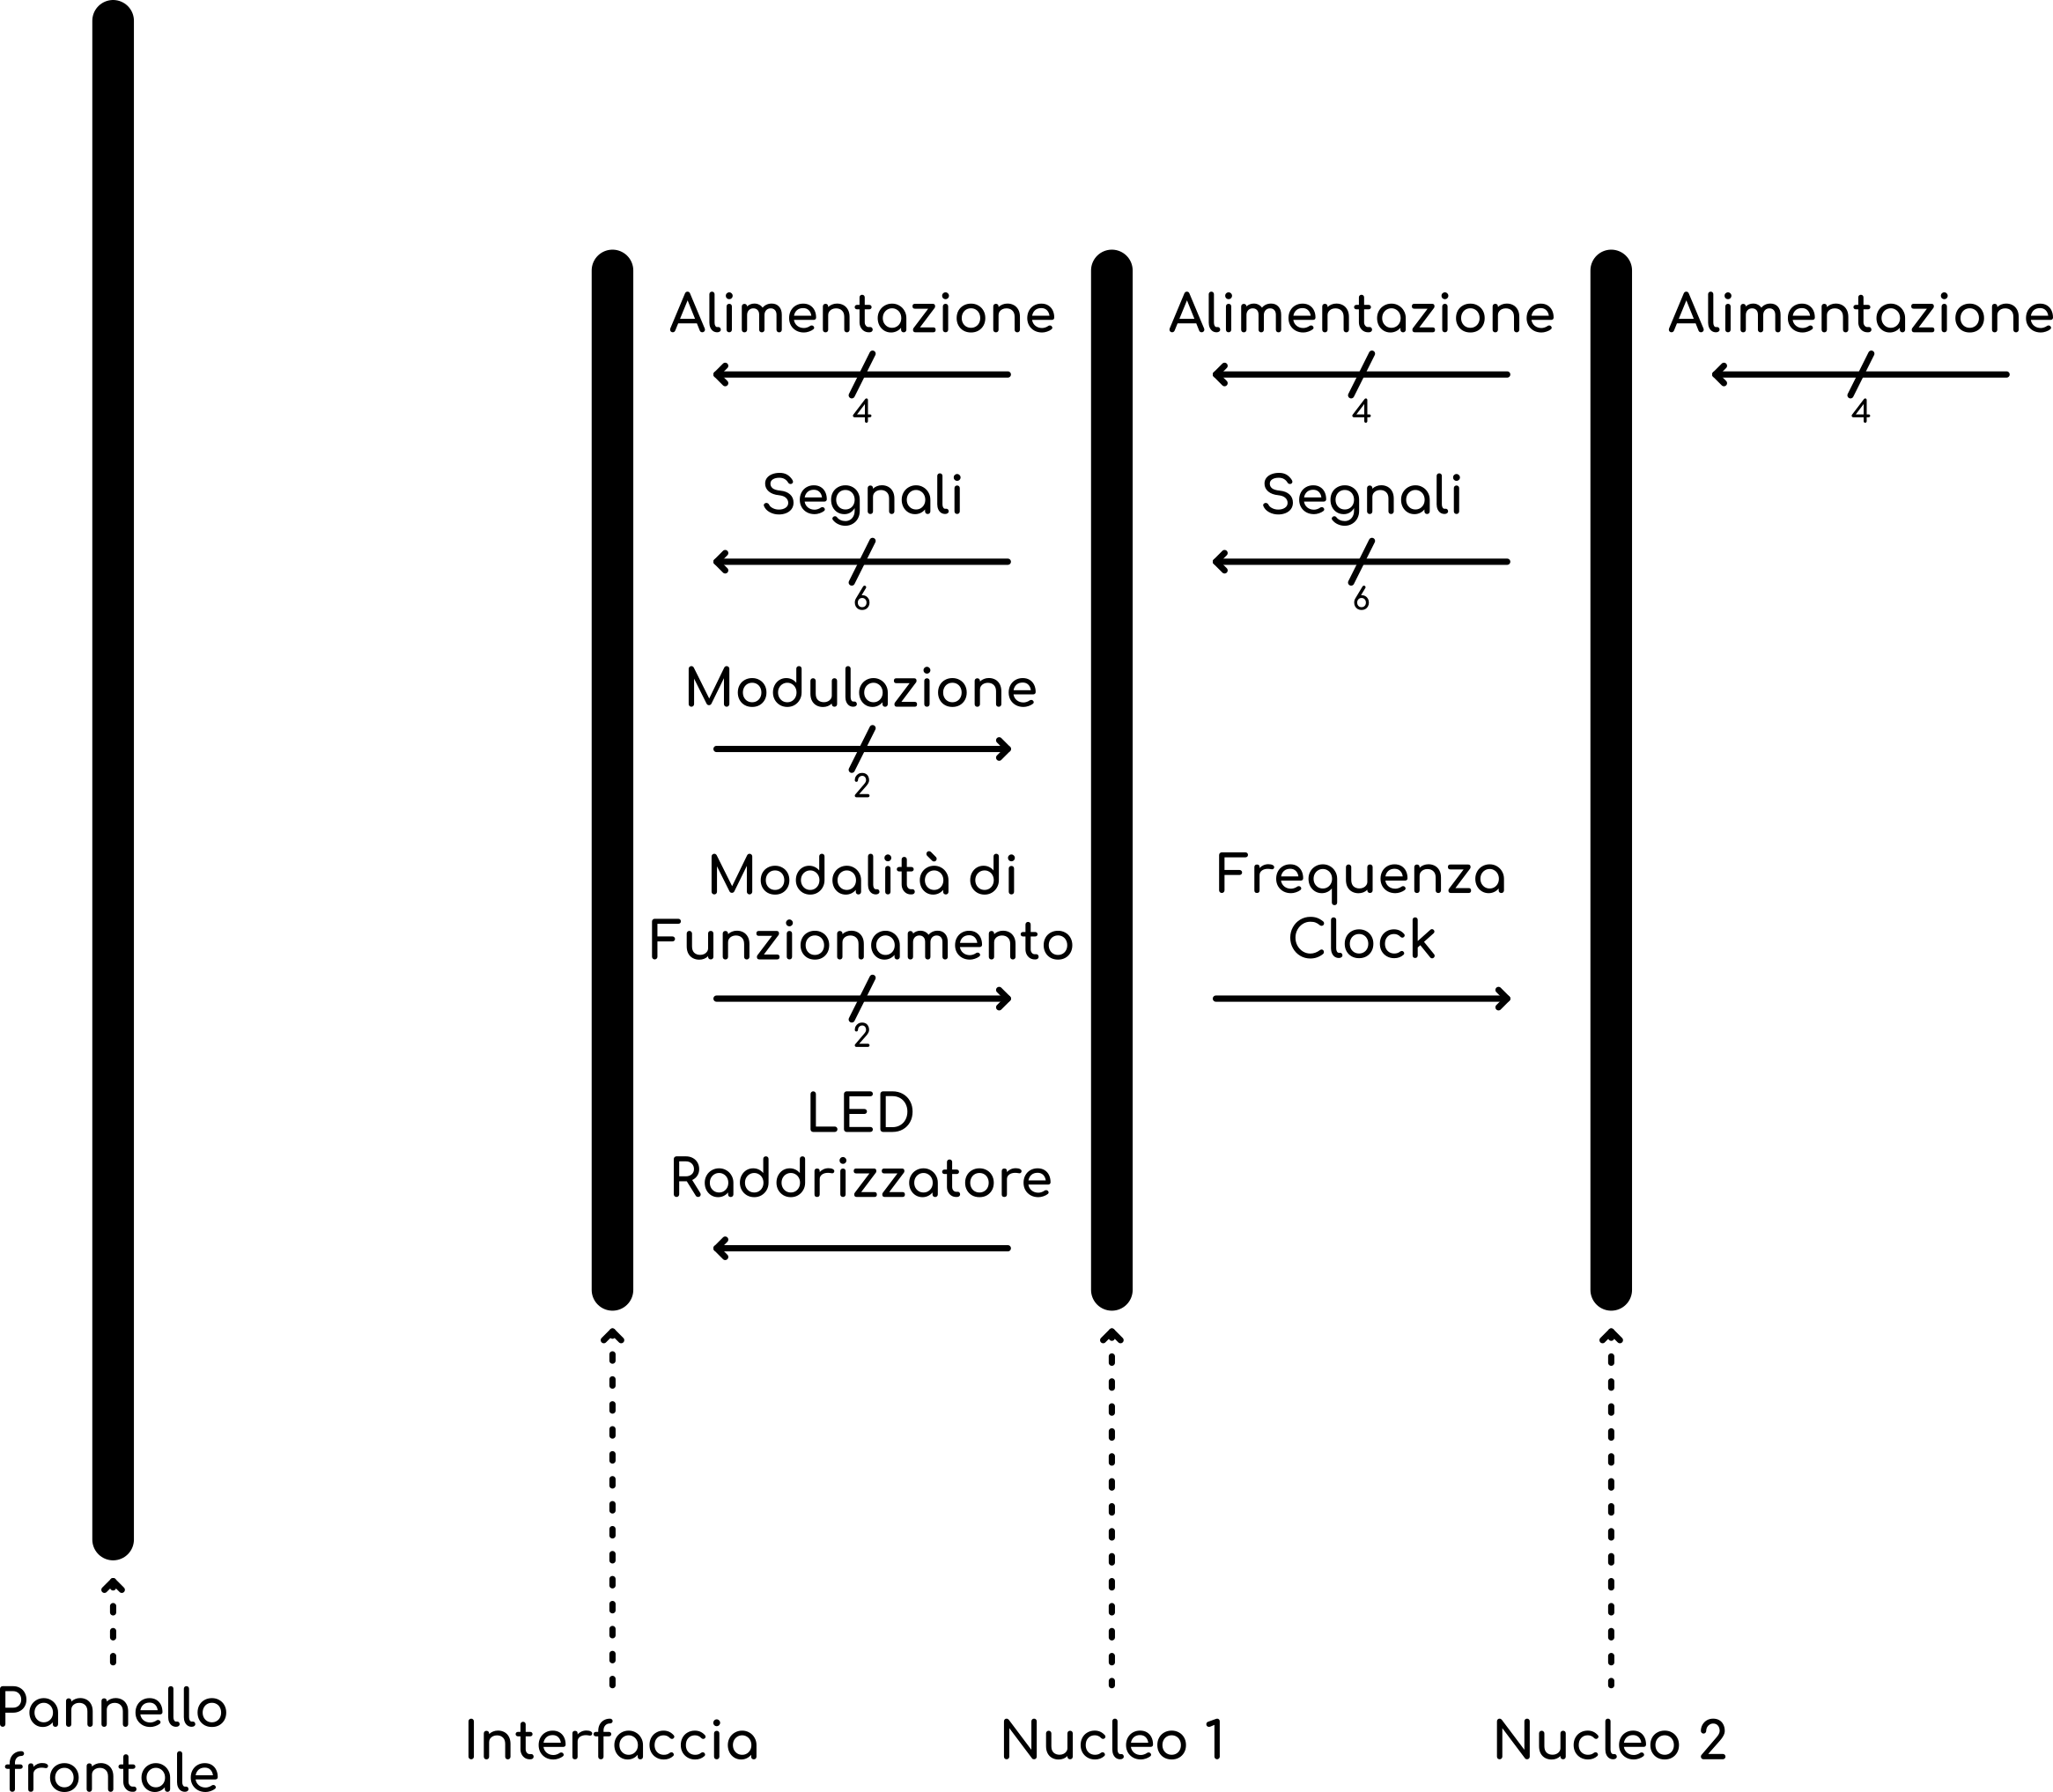
\includegraphics{misc/boards_layout.png}
    \caption{Composizione schede}
    \label{boards_layout}
\end{figure}

Gli schemi elettrici finali utilizzati sono riportati nell'appendice \ref{circuit_diagrams}.

%--------------------------------------------------------------------------------------------

\unsection{Possibili Impieghi del Modulo}

%--------------------------------------------------------------------------------------------

Il modulo in sè non risulta comodamente utilizzabile da solo, e va integrato in un sistema
adeguato assieme a filtri, amplificatori e altri diversi moduli con funzioni varie ed eventuali.
Si riportano allora degli esempi di utilizzo:

\begin{figure}[H]
    \centering
    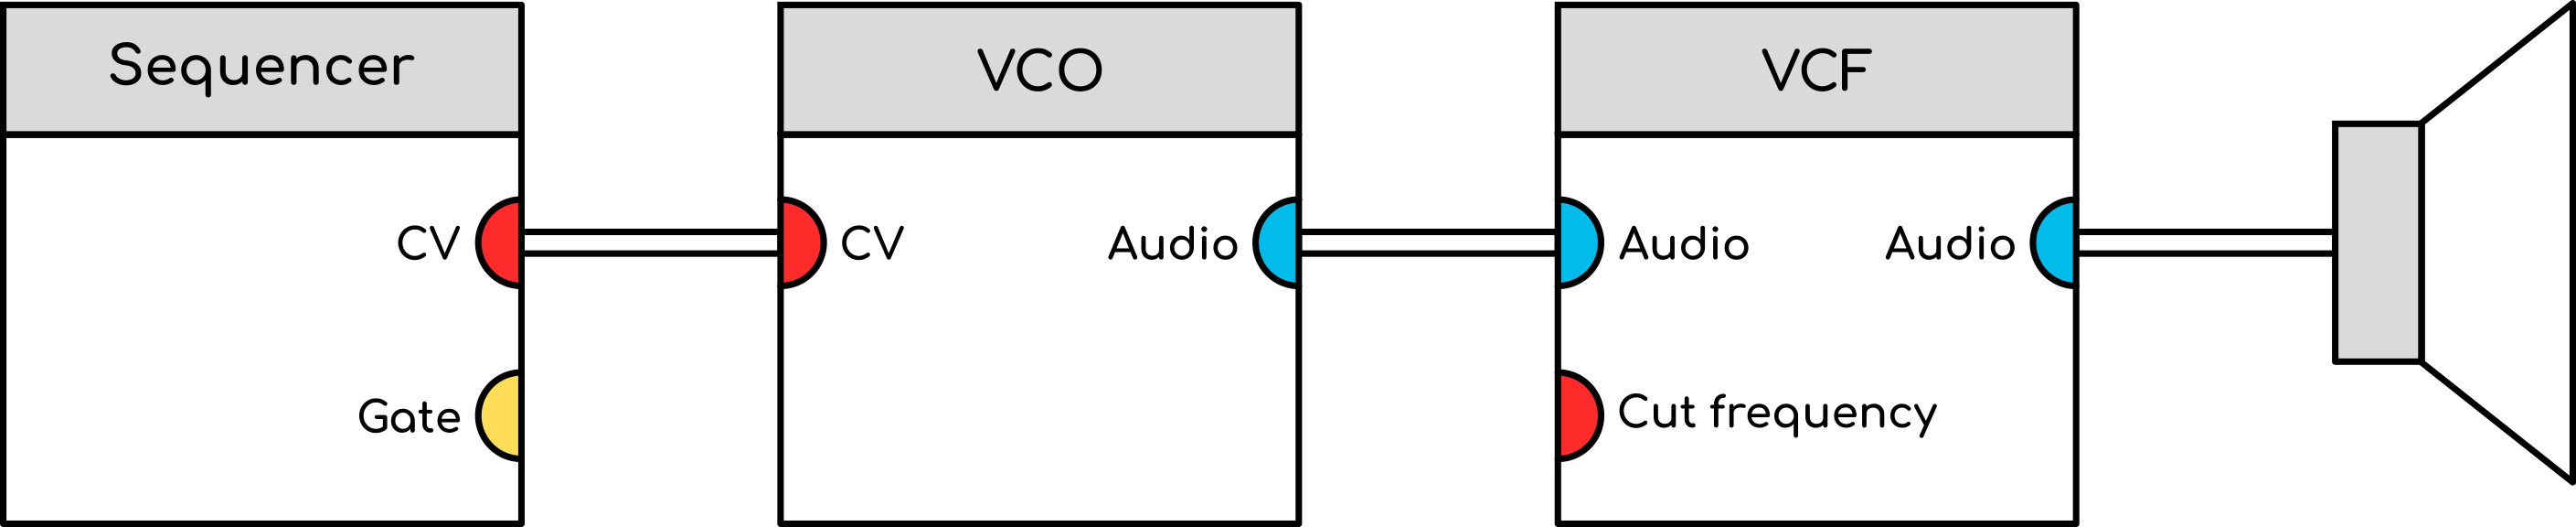
\includegraphics{block_diagrams/example_setup_1.png}
    \caption{Setup d'esempio 1}
    \label{example_setup_1}
\end{figure}

In questo setup si fa uso di un sequenziatore, in grado di fornire un segnale di controllo
che andrà a determinare la nota generata dall'oscillatore. Successivamente il segnale grezzo
generato dall'oscillatore viene modificato da un filtro controllabile in tensione (Voltage
Controlled Filter, o VCF) e poi fornito ad un sistema per la riproduzione del suono.

\begin{figure}[H]
    \centering
    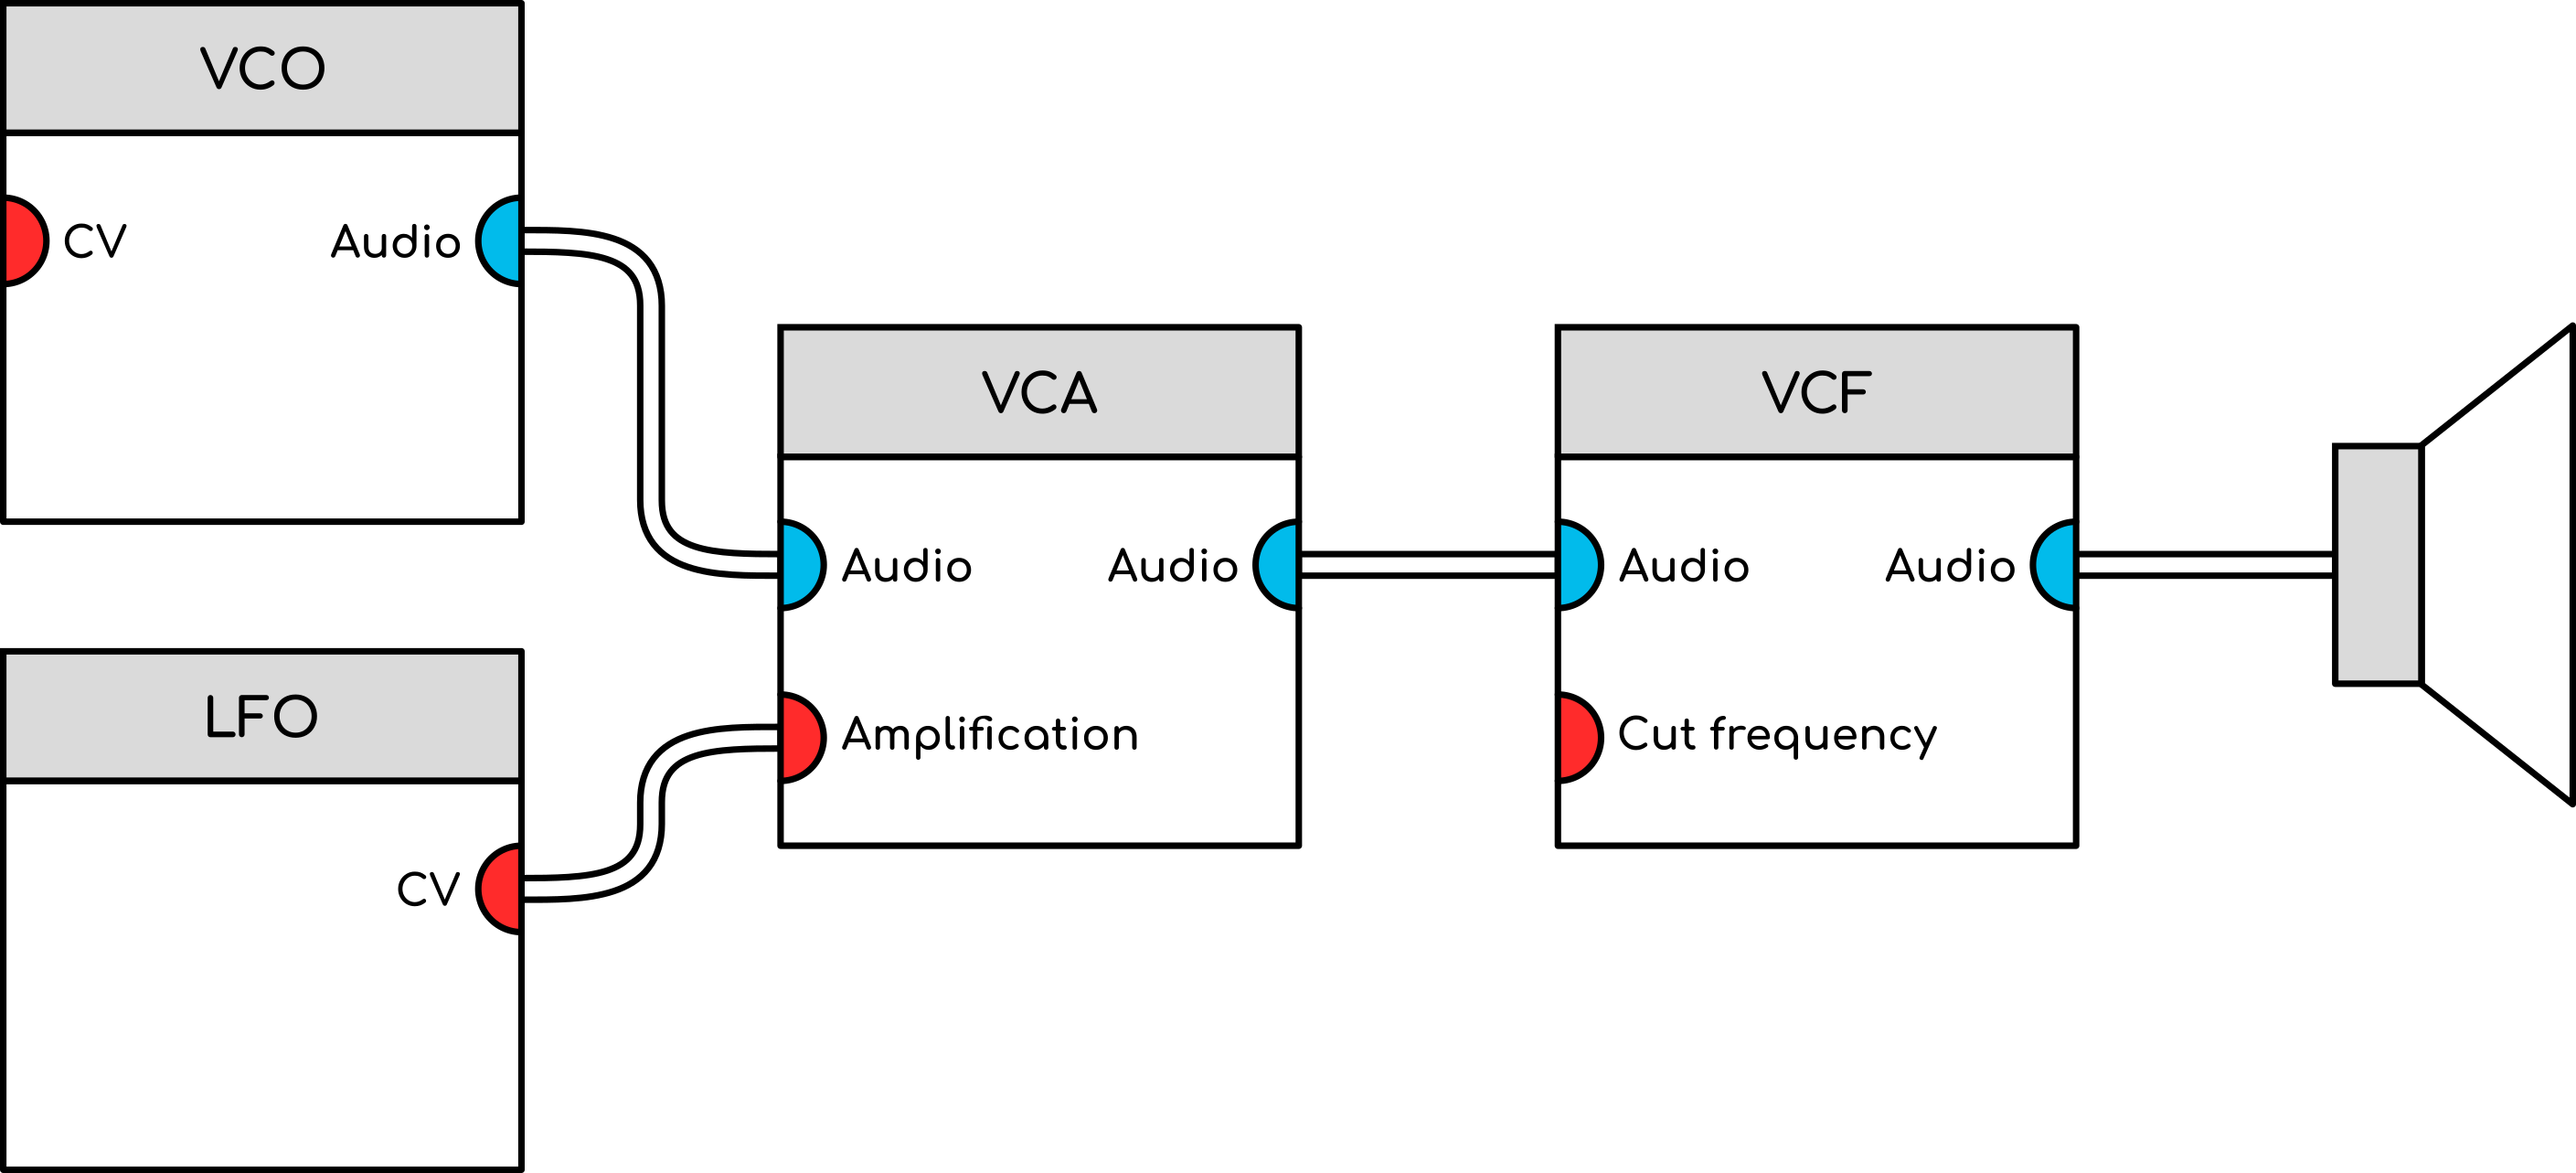
\includegraphics{block_diagrams/example_setup_2.png}
    \caption{Setup d'esempio 2}
    \label{example_setup_2}
\end{figure}

Qui invece, la nota generata rimane costante nel tempo, ma attraverso una combinazione di un
LFO e un amplificatore controllato in tensione (Voltage Controlled Amplifier, o VCA), si
modifica il volume del suono che viene poi filtrato e riprodotto.

\begin{figure}[H]
    \centering
    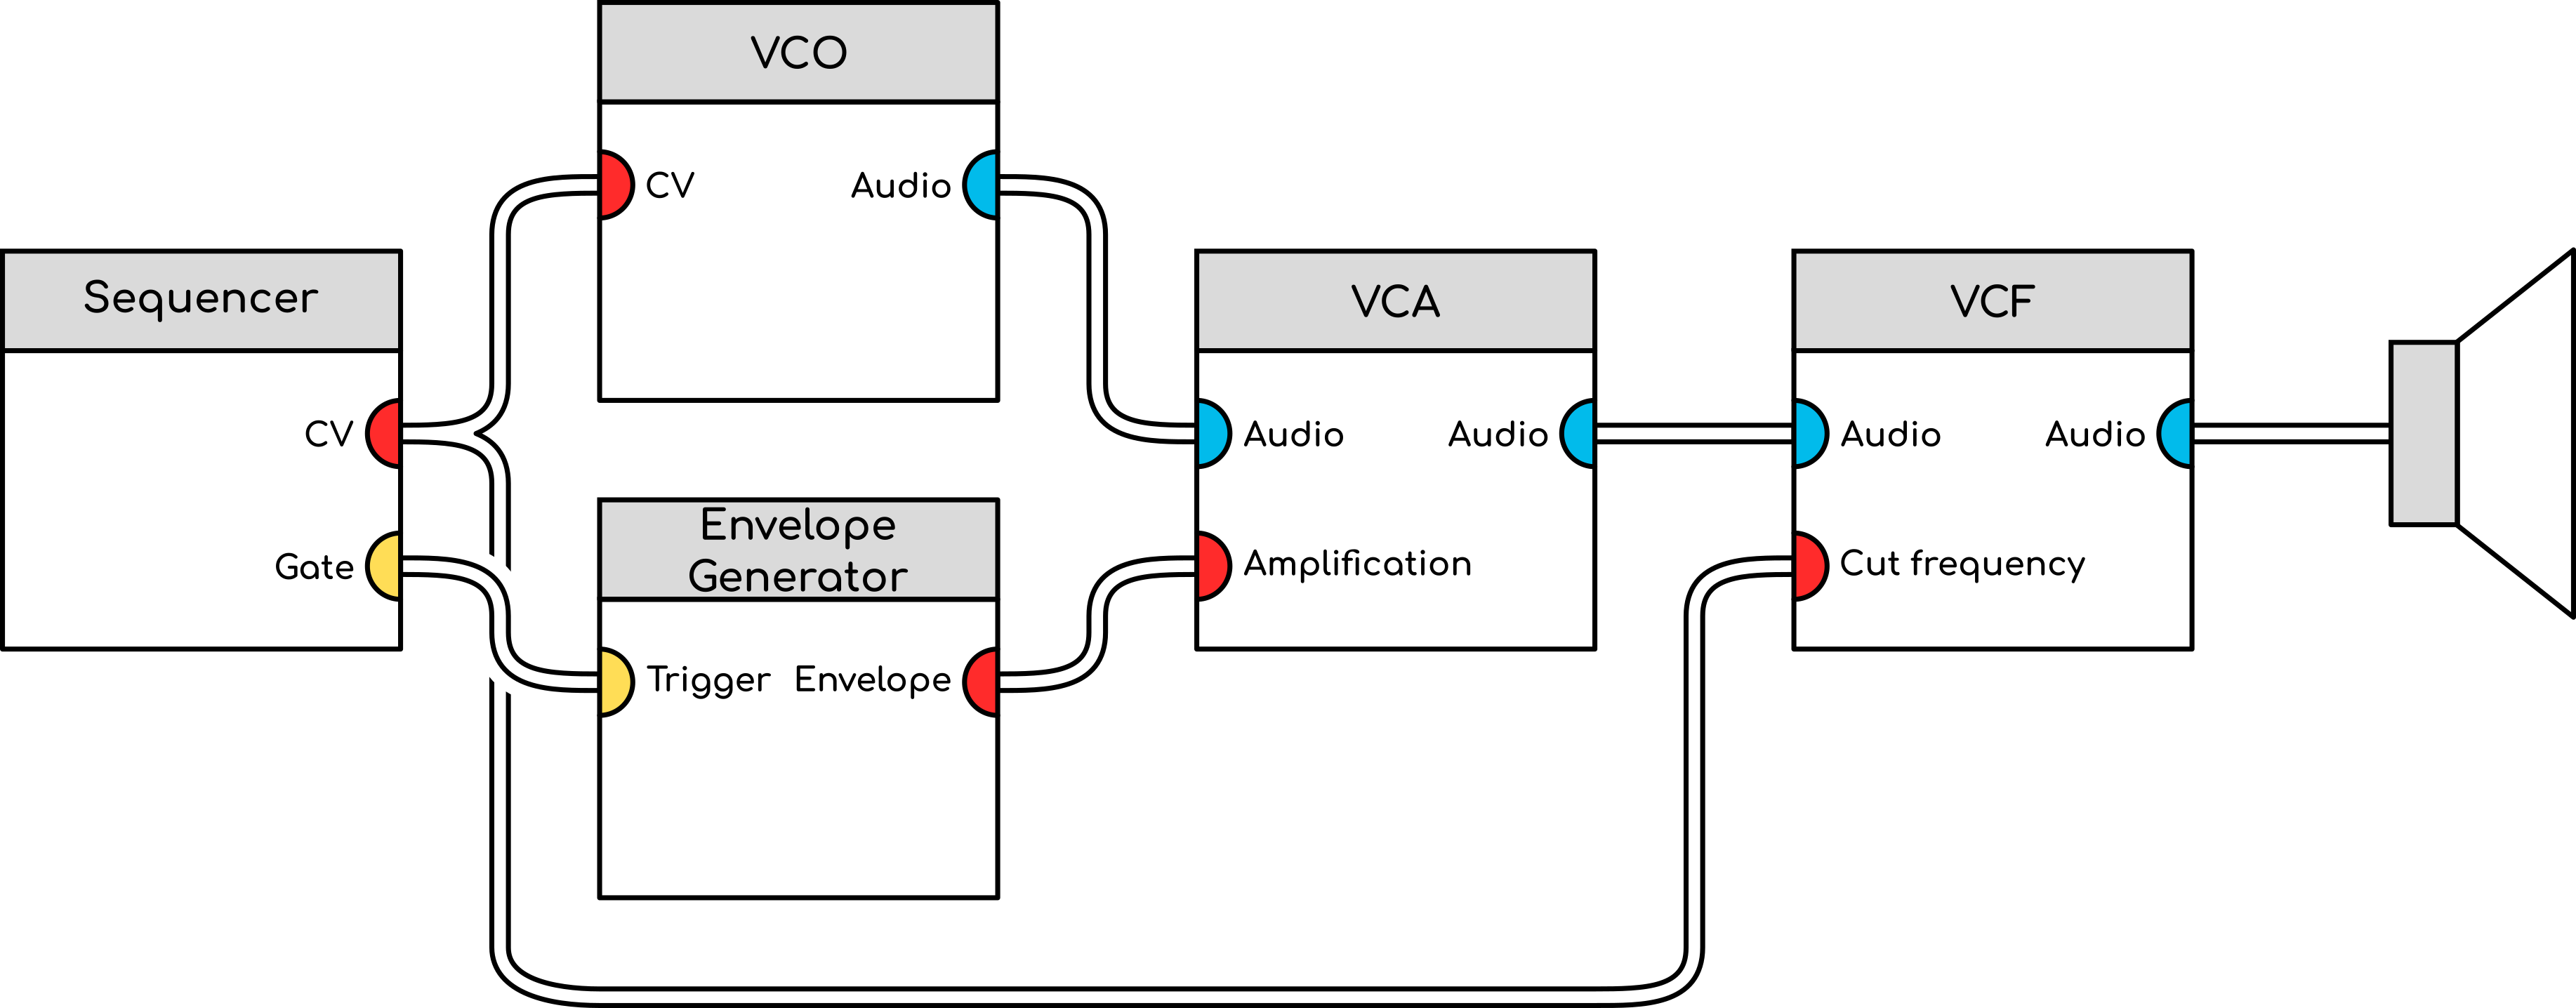
\includegraphics{block_diagrams/example_setup_3.png}
    \caption{Setup d'esempio 3}
    \label{example_setup_3}
\end{figure}

In questo ultimo esempio infine, il sequenziatore determina la nota generata dal VCO e la
frequenza di taglio del filtro. Inoltre la sua uscita gate viene data in pasto ad un generatore
di inviluppo, che si occupa di creare un particolare segnale composto da 4 fasi, ovvero attacco,
discesa, sostegno e rilascio, che viene poi utilizzato per il controllo del volume della nota.
Ancora una volta il segnale viene filtrato e poi riprodotto tramite un adeguato sistema.

%--------------------------------------------------------------------------------------------

\unsection{Considerazioni Finali}

%--------------------------------------------------------------------------------------------

Come già accennato nell'introduzione, la progettazione del modulo sarebbe stata largamente
semplificata se si fossero utilizzati dei microcontrollori, tuttavia l'implementazione
analogica realizzata risulta comunque ottima per lo scopo. È ad ogni modo possibile la
progettazione di una scheda con microcontrollori che realizza le stesse funzioni delle schede
discusse in questa tesi, e che può quindi essere eventualmente sostituita al corrispettivo
analogico, sfruttando la divisione delle schede scelta.

\begin{figure}[H]
    \centering
    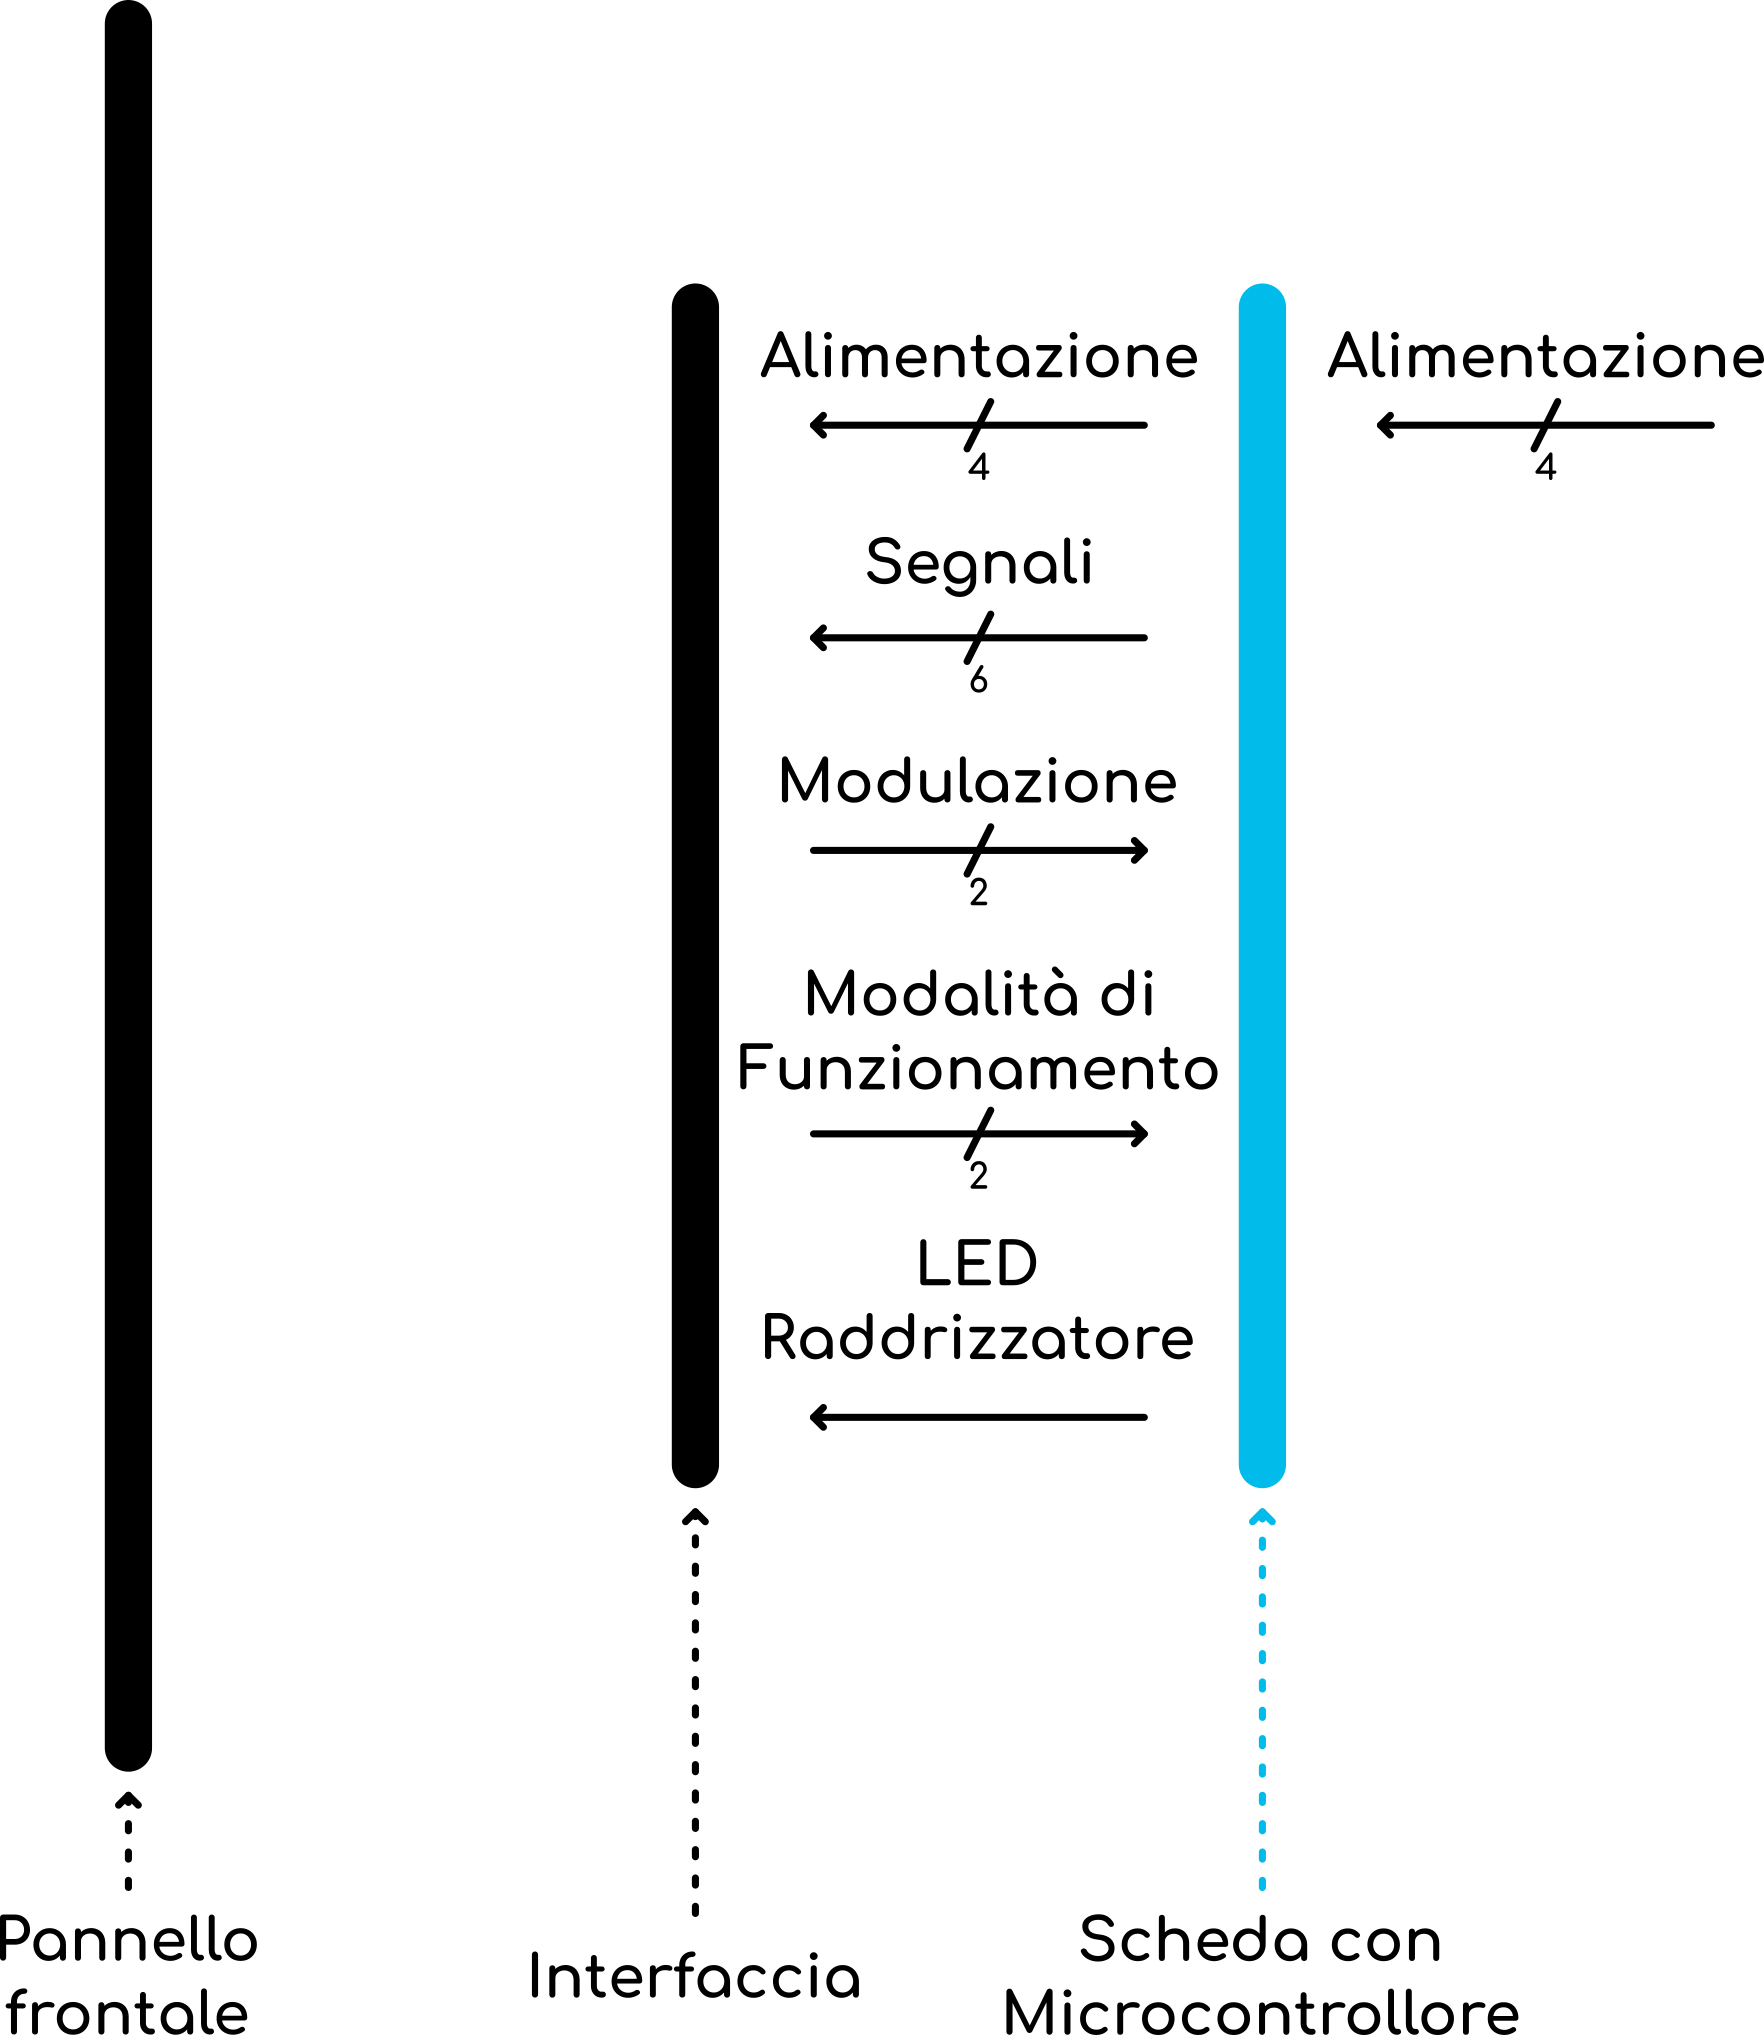
\includegraphics{misc/boards_layout_microcontroller.png}
    \caption{Composizione schede con scheda a microcontrollore}
    \label{boards_layout_microcontroller}
\end{figure}

Per quanto riguarda l'obiettivo, possiamo dire che le specifiche di progetto fornite al
capitolo \ref{introduzione} sono state pienamente rispettate a meno della precisione sulle
note prodotte che risultano in un range leggermente diverso da quello desiderato.

% tabella frequenze per valori di tensione

Tuttavia un aspetto che meriterebbe più attenzioni è l'effetto della temperatura dell'ambiente
sul convertitore lineare-esponenziale, in quanto effettivamente $V_T$ è funzione di essa.
Tale problema potrebbe essere risolto con l'impiego di una termoresistenza adeguatamente
dimensionata, ma non si scenderà oltre in dettaglio.

%--------------------------------------------------------------------------------------------

\newpage
\unsection{Risultato}

%--------------------------------------------------------------------------------------------

Per concludere si riportano delle foto del risultato finale ottenuto.

\begin{figure}[H]
    \centering

    \begin{subfigure}{.5\textwidth}
        \centering
        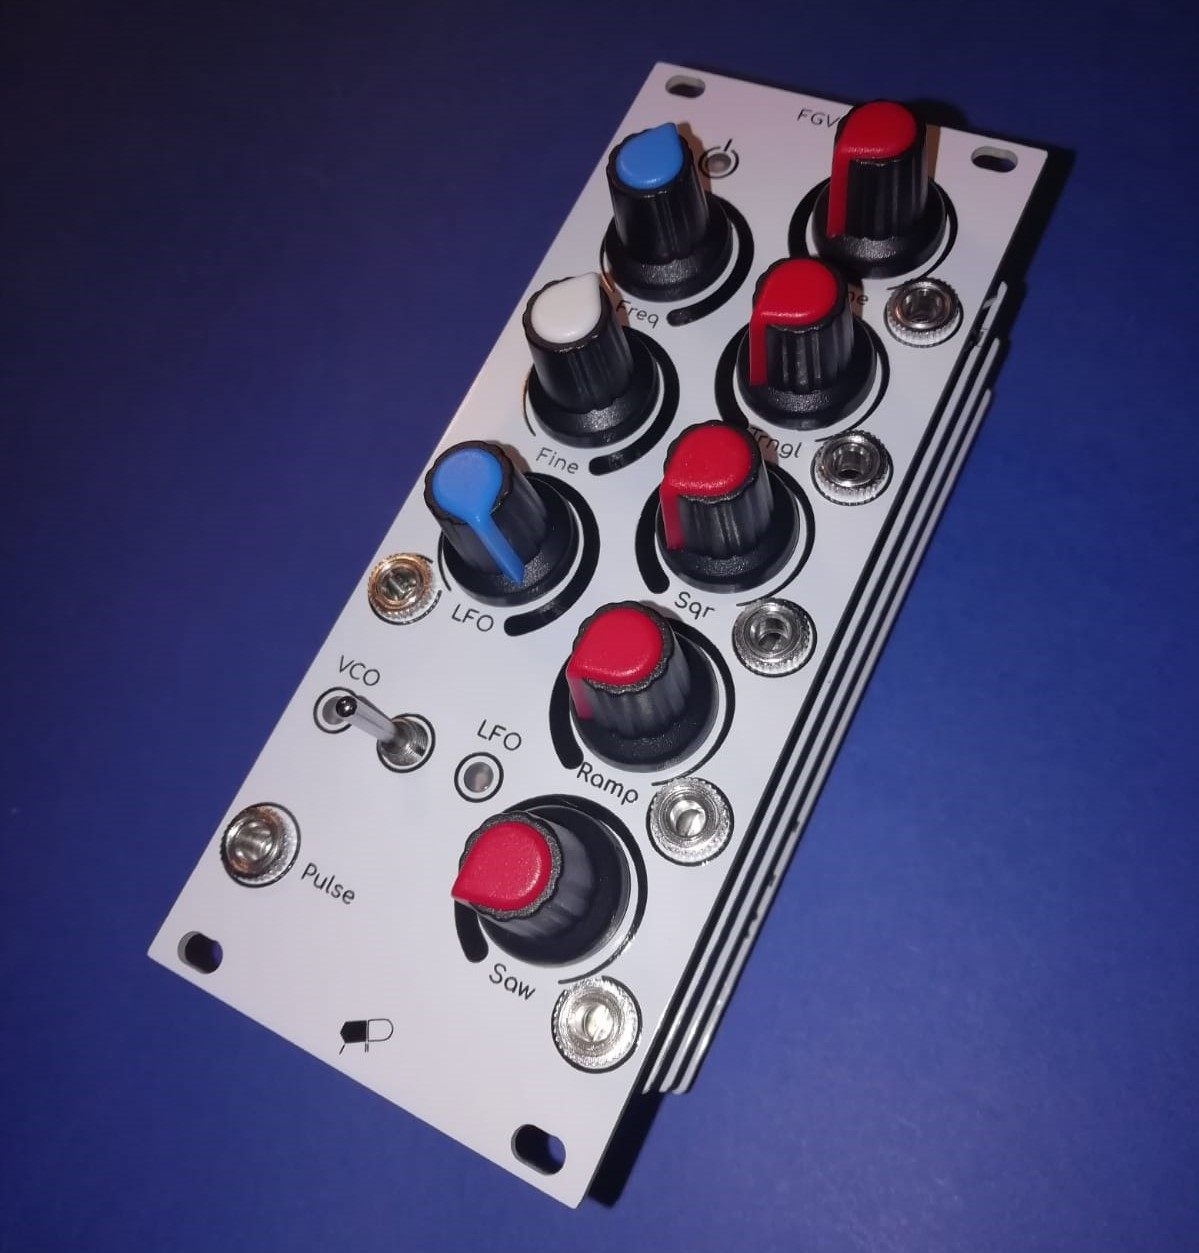
\includegraphics[height = \textwidth]{misc/module_result.jpeg}
        \caption{Modulo realizzato}
        \label{module_result}
    \end{subfigure}%
    \begin{subfigure}{.5\textwidth}
        \centering
        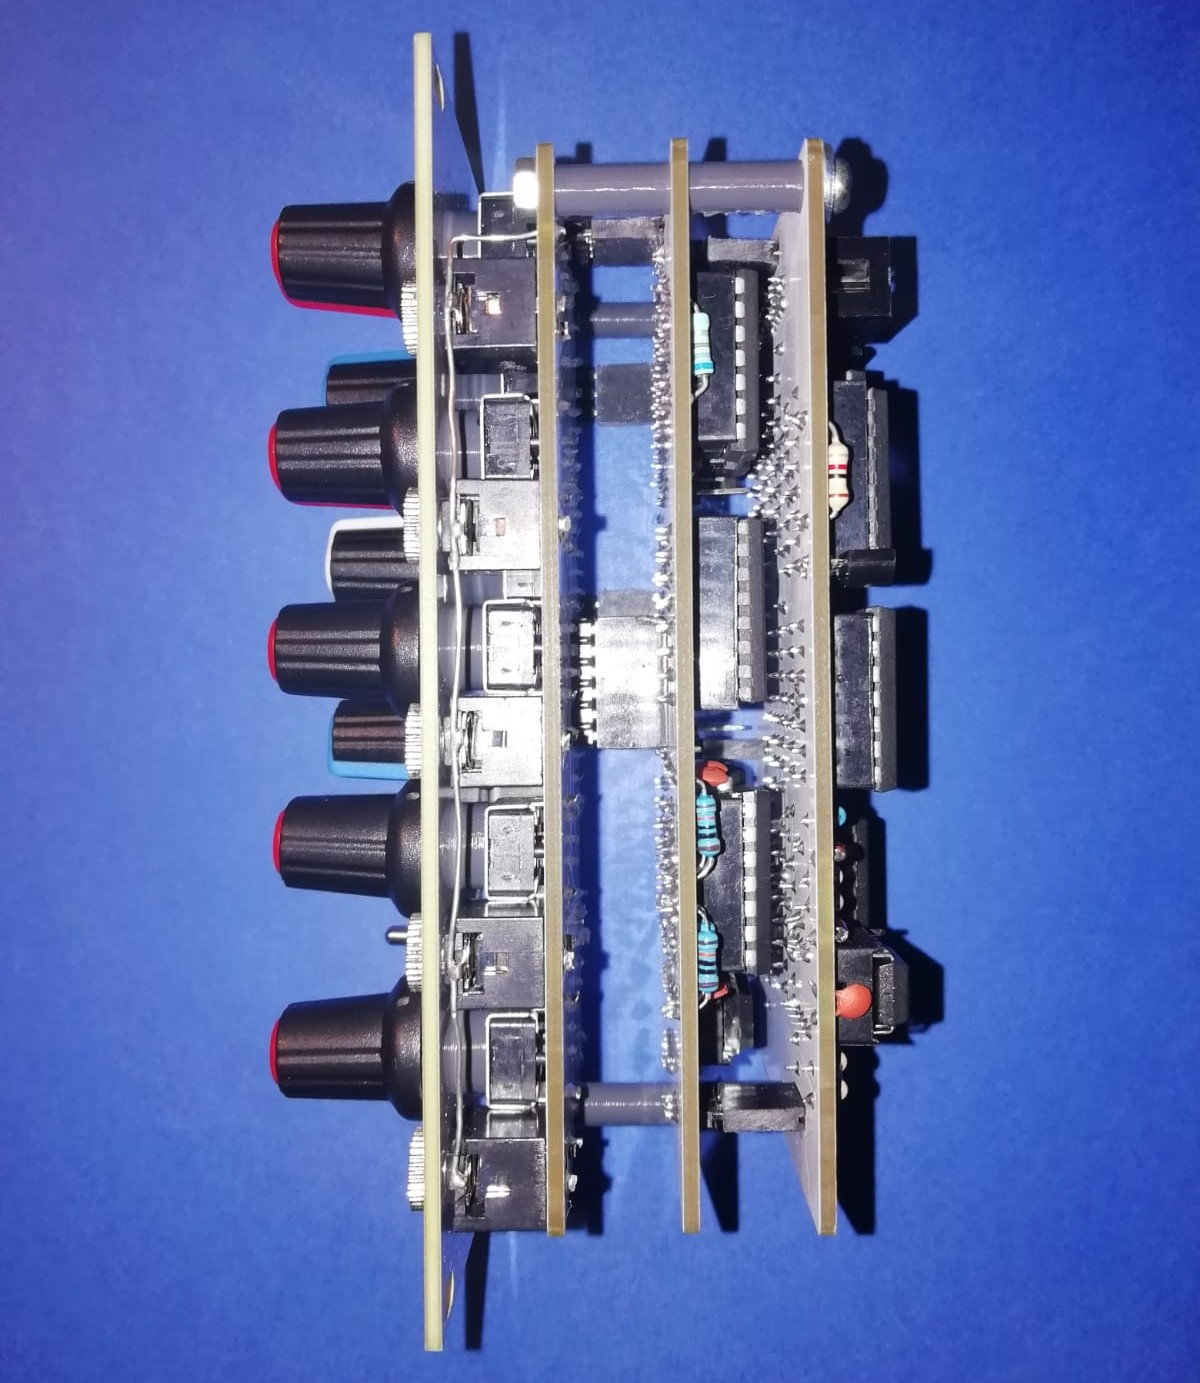
\includegraphics[height = \textwidth]{misc/module_result_side.jpeg}
        \caption{Vista lato}
        \label{module_result_side}
    \end{subfigure}

    \caption*{}
\end{figure}

(foto da sistemare)

%--------------------------------------------------------------------------------------------
